\documentclass[11pt, a4paper]{article}
\usepackage[utf8]{inputenc}
\usepackage{amsmath, amssymb}
\usepackage{graphicx}
\usepackage{hyperref}
\usepackage{xcolor}
\usepackage{listings}
\lstset{
    language=Python,
    basicstyle=\ttfamily\small,
    keywordstyle=\color{blue}\bfseries,
    commentstyle=\color{gray}\itshape,
    stringstyle=\color{orange},
    numberstyle=\tiny\color{gray},
    numbers=left,
    stepnumber=1,
    numbersep=8pt,
    frame=single,
    breaklines=true,
    breakatwhitespace=false,
    showstringspaces=false,
    tabsize=4,
    captionpos=b
}
\usepackage{geometry}
\geometry{margin=1in}

\title{EE 325 Digital Signal Processing \\ Assignment 12: IIR Filter Design – Impulse Invariance and Bilinear Transform}
\author{PERERA J.D.T. \\ E/21/291}
\date{\today}

\begin{document}
\maketitle

\section{1. Impulse Invariance Design}
Given analog low-pass filter: $\displaystyle H_a(s) = \frac{1}{s + 1}$ bounded by $T = 1$ s.

\subsection{(a) Analog impulse response}
Using inverse Laplace:
$$ h_a(t) = \mathcal{L}^{-1}\left\{ \frac{1}{s+1} \right\} = e^{-t} u(t) $$

\subsection{(b) Sampled Sequence and z-Transform}
Sample at $t = nT$ ($T=1$):
$$ h_d[n] = h_a(nT) = e^{-n} u[n] = (e^{-1})^n u[n] $$
The discrete z-transform is:
$$ H_{imp}(z) = \mathcal{Z}\left\{ (e^{-1})^n u[n] \right\} = \frac{1}{1 - e^{-1} z^{-1}} $$

\subsection{(c) Poles, Stability and Mapping}
The digital transfer function $H_{imp}(z)$ possesses a single pole at $z = e^{-1} \approx 0.3679$.
Since $|0.3679| < 1$, the pole resides strictly inside the unit circle, guaranteeing the digital system is \textbf{stable}.
\textbf{Relation:} The process obeys $z = e^{sT}$. The analog pole $s = -1$ cleanly evaluates into $e^{-1(1)} = e^{-1}$ for the digital plane.

\section{2. Bilinear Transform Design}
Applying the bilinear conformal mapping substitute for $T=1$:
$$ s = \frac{2}{T} \frac{1 - z^{-1}}{1 + z^{-1}} = 2 \frac{1 - z^{-1}}{1 + z^{-1}} $$

\subsection{(a \& b) Derivation and Pole Location}
$$ H_{bilin}(z) = H_a\left( 2 \frac{1 - z^{-1}}{1 + z^{-1}} \right) = \frac{1}{ 2 \frac{1 - z^{-1}}{1 + z^{-1}} + 1 } = \frac{1 + z^{-1}}{2(1 - z^{-1}) + 1 + z^{-1}} $$
$$ H_{bilin}(z) = \frac{1 + z^{-1}}{3 - z^{-1}} = \frac{\frac{1}{3} (1 + z^{-1})}{1 - \frac{1}{3}z^{-1}} $$
The system embodies a zero at $z = -1$ and a pole at $z = \frac{1}{3} \approx 0.333$.

\subsection{(c) Qualitative Frequency Mapping Comparison}
\begin{itemize}
    \item \textbf{Impulse Invariance:} Consistently mirrors the standard analog response at low frequencies but suffers strictly from \textbf{aliasing} artifacts toward high frequencies because the entire $j\Omega$ mapping axis infinitely overhangs onto $[-\pi, \pi]$.
    \item \textbf{Bilinear Transform:} Provides an absolute strict mapping mapping $s = \infty$ to $z = -1$ (the rigorous zero induced in our equations proves analytical validity). It flawlessly eliminates all frequency aliasing. Its compromise is severe non-linear \textbf{frequency warping} approaching the Nyquist axis.
\end{itemize}

\section{3. Python – Frequency Response Comparison}
Evaluating the analog frequency parameter against derived digital states utilizing bounds corresponding to equivalence over the $T=1$ span constraints ($\omega = \Omega T = \Omega \implies \omega_{max} = \pi \approx 3.14$).
\begin{figure}[h]
    \centering
    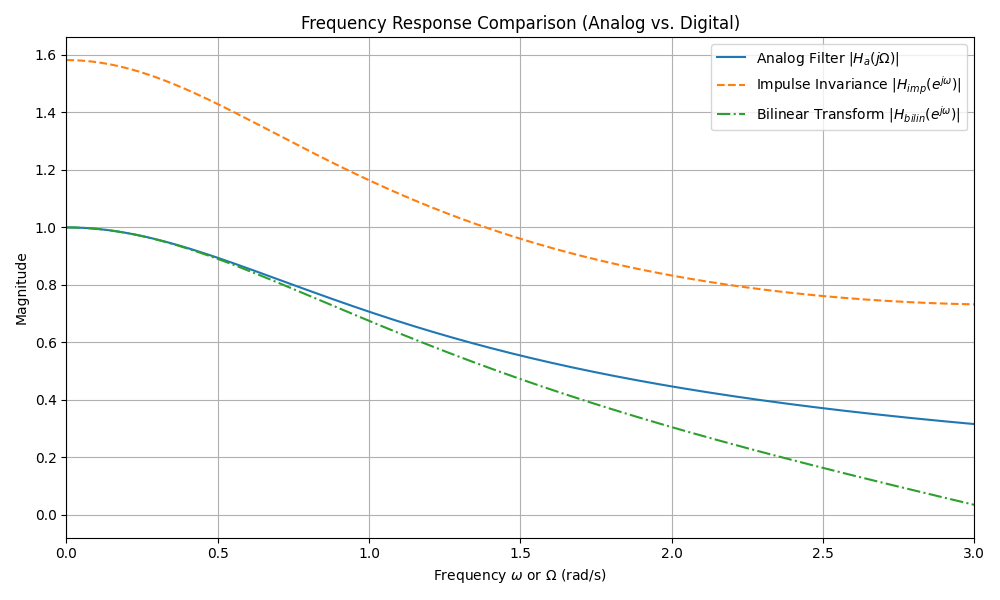
\includegraphics[width=0.8\textwidth]{plots/filter_comparison.png}
    \caption{Simulated Analytical Constraints for the LPF Transformation Structures}
\end{figure}

\textbf{Interpretation Analysis:}
\begin{itemize}
    \item Passband Shape ($\omega \approx 0$): Both the impulse invariance and tracking bilinear transform follow the analytical $|H_a(j\Omega)|$ model cleanly spanning the origin bounds natively tracking 0 dB.
    \item Attenuation / Stopband ($\omega \to \pi$): The Bilinear filter mathematically forces the system cutoff towards the required $z=-1$ Nyquist absolute zero matching perfectly without noise. Impulse Invariance physically fails to reach 0 magnitude at Nyquist because the unbounded continuous spectrum magnitude aliases components above $F_s/2$ downwards into the primary band. 
\end{itemize}

\appendix
\section{Python Source Code}
\textbf{File:} \texttt{assignment12\_iir.py}
\begin{lstlisting}[caption={IIR Design: Impulse Invariance vs. Bilinear Transform -- Assignment 12}]
import numpy as np
import matplotlib.pyplot as plt
import os

def run_assignment12():
    if not os.path.exists('plots'):
        os.makedirs('plots')

    # Analog Filter
    W = np.linspace(0, 3, 1000)
    H_a = 1 / (1j * W + 1)
    mag_Ha = np.abs(H_a)

    # Digital Filters (T=1)
    w = np.linspace(0, np.pi, 1000)

    # Impulse Invariance
    H_imp = 1 / (1 - np.exp(-1) * np.exp(-1j * w))
    mag_Himp = np.abs(H_imp)

    # Bilinear Transform
    H_bilin = (1 + np.exp(-1j * w)) / (3 - np.exp(-1j * w))
    mag_Hbilin = np.abs(H_bilin)

    plt.figure(figsize=(10, 6))
    plt.plot(W, mag_Ha, label='Analog Filter |H_a(jW)|')
    plt.plot(w, mag_Himp, label='Impulse Invariance |H_imp(e^{jw})|', linestyle='--')
    plt.plot(w, mag_Hbilin, label='Bilinear Transform |H_bilin(e^{jw})|', linestyle='-.')
    plt.title('Frequency Response Comparison (Analog vs. Digital)')
    plt.xlabel('Frequency omega or Omega (rad/s)')
    plt.ylabel('Magnitude')
    plt.xlim(0, 3)
    plt.legend()
    plt.grid(True)
    plt.tight_layout()
    plt.savefig('plots/filter_comparison.png')
    print("Assignment 12 plot saved.")

if __name__ == '__main__':
    run_assignment12()
\end{lstlisting}

\end{document}
